In der statischen Kennlinie wird der Ausgang über dem Eingang dargestellt. Bei einem linearen System (unten $u$ oben $y$) ist die statische Kennlinie eine Ursprungsgerade, deren Anstieg der statischen Verstärkung entspricht. 
Die statische Verstärkung $K$ kann aus $G(0)=K$ berechnet werden. Sie ist bei Systemen mit D-Verhalten 0 und bei Systemen mit I-Verhalten unendlich. Mit anderen Worten, Systeme mit I-Verhalten haben keine Kennlinie.\\
In der statischen Kennlinie ist keinerlei Dynamik zu erkennen und die Information über Pole, Nullstellen, etc. fehlen. Sie ist somit die schwächste der Modellbeschreibungen. 
Allerdings ist sie dafür einfach zu bestimmen. Man stellt einen konstanten Wert $u$ ein, wartet bis die Eigenvorgänge abgeklungen 
%(bis es eingeschwungen ist) 
sind und liest den $y$-Wert ab. Diesen Punkt trägt man in das Diagramm ein und wiederholt das ganze für mehrere Punkte.\\
In der Praxis werden sich häufig nicht ideale Geraden ergeben. Bei Öfen verringert sich der Anstieg beispielsweise bei hohem $u$. Der Praktiker ließt aus der statischen Kennlinie ab, wie gut seine Annahme eines linearen Modells ist. Sie ist gut in einem Bereich, in dem eine Geradenapproximation akzektabel ist (wenn sie einer Gerade ähnelt). Bei einem Mehrgrößensystem mit zwei Eingängen und zwei Ausgängen wählt man häufig die folgende Darstellung: Entweder zwei Einzeldiagramme, oder ein Verbunddiagramm (zwei Eingänge ein Ausgang: Üblicherweise keine 3D-Darstellung, sondern Transistorkennlinien). Bei Systemen mit zwei Eingängen 
%wird häufig eine Eingangsvariable durch Kennlinienscharen diskretisiert/
wählt man häufig die Darstellung mit Kennlinienscharen, wobei beispielsweise $u_{1}$ die reellen Zahlen darstellt und $u_{2}$ den Scharparameter darstellt.\\
%Indem man alle Ableitungen gleich Null setzt und eine Beziehung zwischen den y und u herstellt. Gegebenenfalls muss x eliminiert werden (lineares Gleichungssystem).
Da unser System nur einen Eingang und einen Ausgang besitzt, reicht demnach folgende Darstellung, welche sich durch folgende Matlab-Befehle erzeugen lässt:\\
\hspace*{0.5cm}\texttt{syms u}\\
\hspace*{0.5cm}\texttt{fplot(dcgain(sys)*u, [0 100])}\\
Die statische Kennlinie unseres Systems sieht aus wie folgt:
\begin{figure}[H]
    \centering
    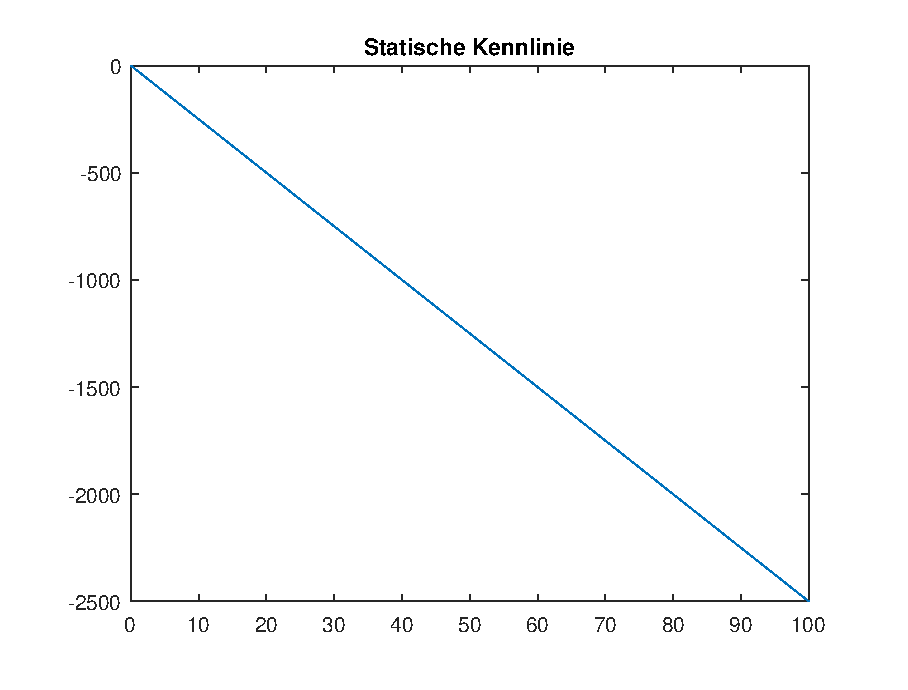
\includegraphics[width=10cm]{images_2/Rest/statische_kennline.eps}
    \caption{Statische Kennlinie}
\end{figure}